\esSezione{Sistema ROM + M su board}\label{sec:esercizio2-2}

\begin{traccia}
Sintetizzare ed implementare su board il progetto del sistema ROM+M sviluppato al punto 2.1, utilizzando gli switch per fornire l'indirizzo della ROM da cui leggere i valori da trasformare e i led per visualizzare i 4 bit di uscita.
\end{traccia}

\progetto

Il sistema $S$ è già stato progettato e descritto nell'esercizio~\ref{sec:esercizio2-1}: non viene modificato. Per portarlo su board si aggiunge un solo componente, un top module che espone le porte fisiche della scheda e le collega a quelle di \texttt{systemS}. Il sistema è puramente combinatorio, quindi usiamo solo switch e led.

\implementazione

I componenti \texttt{rom16\_8}, \texttt{systemM} e \texttt{systemS} sono quelli presentati nell'esercizio~\ref{sec:esercizio2-1} (listati~\ref{lst:esercizio2-1:rom16-8}, \ref{lst:esercizio2-1:systemm} e~\ref{lst:esercizio2-1:systems}) e non vengono ivi riportati.

L'entità \texttt{systemS\_tl} ha l'ingresso \texttt{SW} e l'uscita \texttt{LED}, entrambi a 4 bit. L'architettura \texttt{structural} non dichiara segnali interni e contiene una sola istanza di \texttt{systemS}, con etichetta \texttt{SYSTEM\_S}, il cui port mapping per nome collega \texttt{input} a \texttt{SW} e \texttt{output} a \texttt{LED}. 

\vhdlfile{esercizio2-2/systems_tl.vhd}{Implementazione del top module su board}{lst:esercizio2-2:systems-tl}

\sintesiboard

Gli interruttori \texttt{SW[0]}--\texttt{SW[3]} della scheda Nexys A7-100T forniscono l'indirizzo $A$ della ROM, mentre i LED \texttt{LED[0]}--\texttt{LED[3]} mostrano il valore a 4 bit prodotto da $M$. Cambiando la configurazione degli interruttori si ottiene sui LED il risultato dell'AND tra coppie di bit adiacenti del contenuto della locazione selezionata.

% TODO: foto della scheda e verifica del comportamento su board, non disponibili nel progetto

Nel file dei constraint sono state decommentate le seguenti righe, che assegnano ai quattro interruttori e ai quattro LED i rispettivi pin della scheda, con standard di I/O \texttt{LVCMOS33}.

\xdcfile{esercizio2-2/vincoli.xdc}{Constraint}{lst:esercizio2-2:vincoli}

\begin{figure}[H]
  \centering
  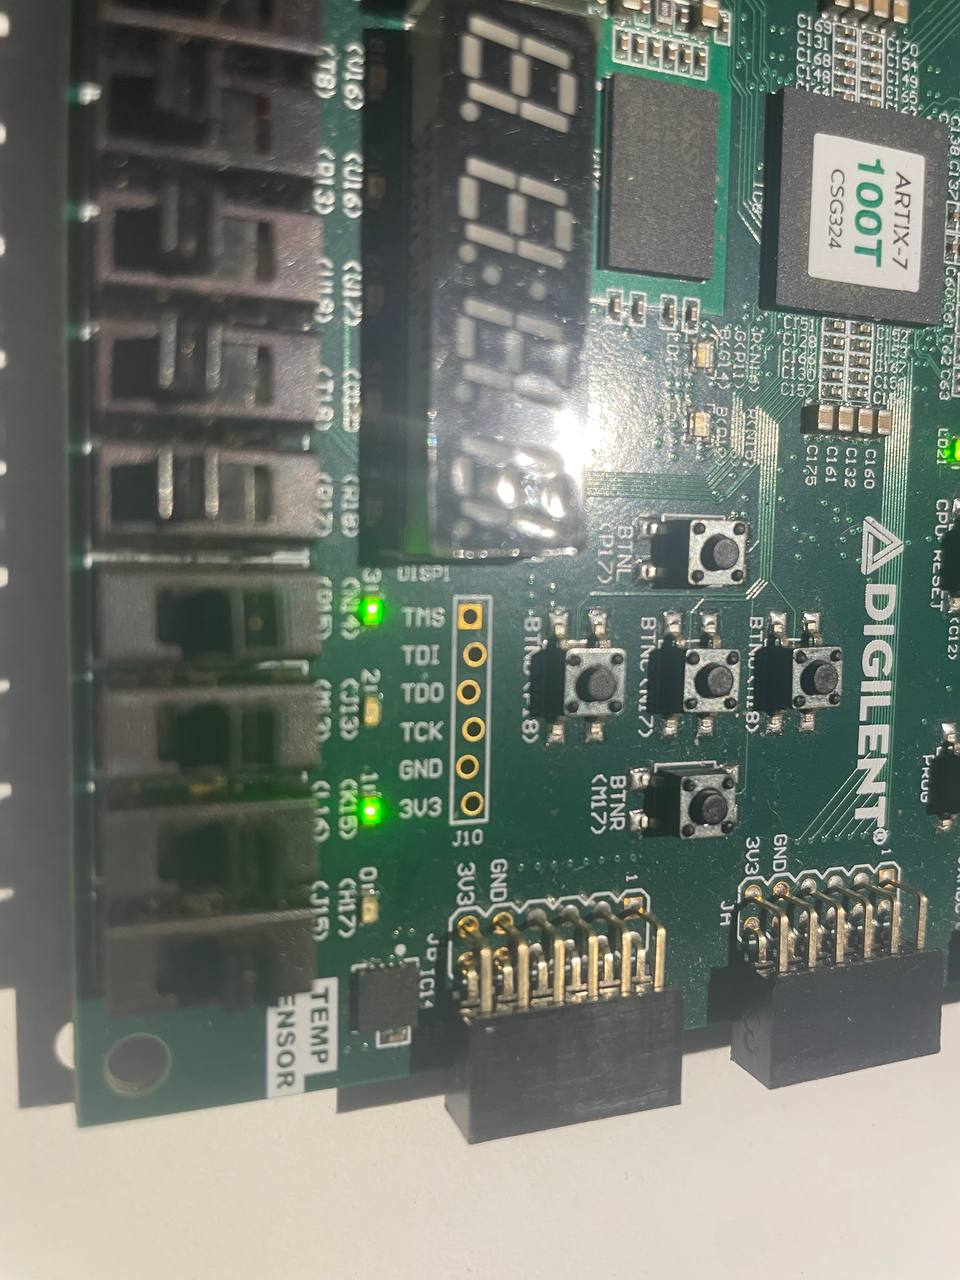
\includegraphics[width=0.7\linewidth]{figure/esercizio2-2/irl.jpg}
  \caption{Realizzazione sistema ROM + M}
  \label{fig:esercizio2-2:realizzazione}
\end{figure}
